\documentclass[tikz, 12pt]{article}
\usepackage[margin=0.7in]{geometry}
\usepackage{amsmath}
\usepackage[makeroom]{cancel}
\usepackage{graphicx}
\usepackage[utf8]{inputenc}
\usepackage{ stmaryrd }
\usepackage{multicol}
\usepackage{tasks}
\usepackage{tabularx}
\usepackage{tasks}
 \usepackage{vwcol} 
 \usepackage{booktabs}
 \usepackage{tabularray}
 \usepackage{pgfplots}
 \usepackage{fancyhdr}
 \usepackage{xcolor}
 \usepackage{soul}
 \usepgflibrary{plotmarks}
\def\newline{\hfill \break}
\def\({\left(}
\def\){\right)}
\def\ddx{\frac{d}{dx}}
\def\[{\left[}
\def\]{\right]}
\def\ddy{\frac{dy}{dx}}
\setul{0.5ex}{0.2ex}
\setulcolor{red}
\begin{document}
\begin{flushleft}
\begin{large}\textbf{Section 4.1: Minimum and Maximum Values (Part a)}\end{large} \\
\newline
In this section we will learn how to use the derivative of a function to find its maximum and
minimum values. \\
Furthermore, we will learn conditions which guarantee that a function has extreme values, and
methods for determining their location. \\
\newline
\textbf{Warm Up} \\
\newline
Suppose the graph of a function $f$ below. What is the \ul{highest} and \ul{lowest} values of $f$. \\
\newline
\begin{center}
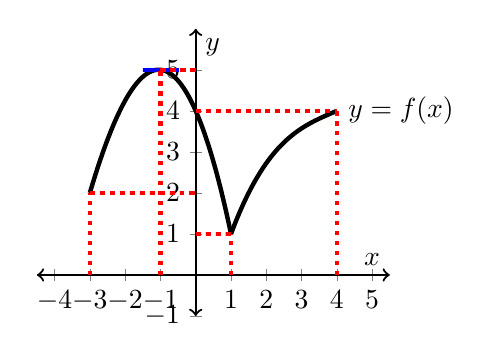
\begin{tikzpicture}
		\begin{axis} [
		width = 0.5\textwidth,
		axis x line=middle,
                   axis y line=middle,
		ymin = -1, ymax = 6,
		xmin = -4.5, xmax = 5.5,
		xtick={-4, -3, -2, -1, 0, 1, 2, 3, 4, 5
        		},
        		ytick = {-1, 0, 1, 2, 3, 4, 5},
        		xlabel = {$x$},
        		ylabel = {$y$},
        		every axis plot/.append style={ultra thick},
        		clip = false,
        		axis line style = {<->, thick},
		]
			\addplot [
			black,
			samples = 200,
			domain = -3:1,
			]
			{((5*(x+3)*(x+0)*(x-1))/4)+((2*(x+1)*(x+0)*(x-1))/-24)+((4*(x+1)*(x+3)*(x-1))/-3)+((1*(x+1)*(x+3)*(x+0))/8)};
			
			\addplot [
			blue,
			samples = 200,
			domain = -1.5:-.5,
			]
			{5};
			
			\addplot [
			black,
			samples = 200,
			domain = 1:4,
			]
			{((1*(x-1.5)*(x-2.25)*(x-4))/-1.875)+((2*(x-1)*(x-2.25)*(x-4))/0.9375)+((3*(x-1)*(x-1.5)*(x-4))/-1.6406)+((4*(x-1)*(x-1.5)*(x-2.25))/13.125)} node[right]{$y = f(x)$};
			
			\addplot [red, dotted] coordinates {(-3, 0) (-3, 2)};
			\addplot [red, samples = 200, domain = -3:0, dotted]{2};
			
			\addplot [red, dotted] coordinates {(-1, 0) (-1, 5)};
			\addplot [red, samples = 200, domain = -1:0, dotted]{5};
			
			\addplot [red, dotted] coordinates {(1, 0) (1, 1)};
			\addplot [red, samples = 200, domain = 0:1, dotted]{1};
			
			\addplot [red, dotted] coordinates {(4, 0) (4, 4)};
			\addplot [red, samples = 200, domain = 0:4, dotted]{4};
		\end{axis}
	\end{tikzpicture}
\end{center}
	\begin{flalign*}
	\text{The Highest} &= \text{Largest Value} & f(-1) &= 5 \text{ The largest value of } f\\
	\text{The Lowest} &= \text{Smallest Value} & f(1) &= 1 \text{ The smallest value of } f
	\end{flalign*}
	$$\text{Domain }f\text{:} [-3,4]$$ \\
	\begin{flalign*}
	\text{The maximum value is } 5 \text{ at } x &= -1 \\
	\text{The minimum value is } 1 \text{ at } x &= 1
	\end{flalign*}
	\fbox{
	\parbox{\textwidth}{
	\newline
		\textbf{Definition} \\
		\newline
		Let \ul{$c$} be a number \ul{in the domain $D$} of a function $f$.
		\begin{itemize}
		\item{If $f(c) \ge f(x)$ for all $x$ in $D$, then $f(c)$ is an \textbf{\ul{absolute maximum}} (or \textbf{\ul{global maximum}}) value.}
		\item{If \color{red}\fbox{\color{black}$f(c) \le f(x)$} \color{black} for all $x$ in $D$, then $f(c)$ is an \textbf{\ul{absolute minimum}} (or \textbf{\ul{global minimum}}) value.}
		\end{itemize}
		\newline
		The minimum and maximum values of $f$ are known as \textbf{\ul{extreme values}} or just \textbf{extrema}.
	}}
	\clearpage
	How do we find absolute extrema? \\
	\vspace{4ex}
	\begin{tblr}{
	width=\textwidth, 
	rows = {halign = c, valign = m}, colspec={X X},}
	{\begin{tikzpicture}
		\begin{axis} [
		width = \linewidth,
		axis x line=middle,
                   axis y line=middle,
		ymin = -1, ymax = 3,
		xmin = -2, xmax = 2,
		xtick={-1, 0, 1},
        		ytick = {0, 1, 2},
        		xlabel = {$x$},
        		ylabel = {$y$},
        		every axis plot post/.append style={ultra thick},
        		clip = false,
        		axis line style = {<->, thick},
        		title = {$f(x) = x^2 + 1 \text{ on } \(-\infty, \infty\)$},
		]
			\addplot [
			black,
			samples = 200,
			domain = -1:1,
			style={<->}
			]
			{x^2 + 1};
			\addplot[mark=*] coordinates {(0,1)};
			
			\addplot [
			red,
			dotted,
			samples = 200,
			domain = -0.5:0.5,
			]
			{1} node[right]{$f'(0) = 0$};
			
			\node[red, thick] (source) at (axis cs:-1.5,0.5){abs min is $1$ at $x=0$};
       			\node (destination) at (axis cs:0, 1){};
       			\draw[red, thick, ->](source)--(destination);
	\end{axis}
	\end{tikzpicture} \\
	There is no abs max} & 
	{\begin{tikzpicture}
		\begin{axis} [
		width = \linewidth,
		axis x line=middle,
                   axis y line=middle,
		ymin = -1, ymax = 3,
		xmin = -2, xmax = 2,
		xtick={-1, 0, 1},
        		ytick = {0, 1, 2},
        		xlabel = {$x$},
        		ylabel = {$y$},
        		every axis plot post/.append style={ultra thick},
        		clip = false,
        		axis line style = {<->, thick},
        		title = {$f(x) = x^2 + 1 \text{ on } \[0, 1\]$},
		]
			\addplot [
			black,
			samples = 200,
			domain = 0:1,
			]
			{x^2 + 1};
			\addplot[mark=*] coordinates {(0,1)};
			\addplot[mark=*] coordinates {(1,2)};
			
			\addplot [
			red,
			dotted,
			samples = 200,
			domain = 0:1,
			]
			{2};
			
			\node[red, thick] (source) at (axis cs:-1.5,0.5){abs min is $1$ at $x=0$};
       			\node (destination) at (axis cs:0, 1){};
       			\draw[red, thick, ->](source)--(destination);
			
			\node[red, thick] (source) at (axis cs:2,3){abs max is $2$ at $x=1$};
       			\node (destination) at (axis cs:1, 2){};
       			\draw[red, thick, ->](source)--(destination);
       			\addplot [red, dotted] coordinates {(1, 0) (1, 2)};
	\end{axis}
	\end{tikzpicture} \\
	The abs max and min occur at the endpoints} \\
	\end{tblr} \\
	\vspace{10ex}
	\begin{tblr}{
	width=\textwidth, 
	rows = {halign = c, valign = m}, colspec={X X}}
	{\begin{tikzpicture}
		\begin{axis} [
		width = \linewidth,
		axis x line=middle,
                   axis y line=middle,
		ymin = -1, ymax = 3,
		xmin = -2, xmax = 2,
		xtick={-1, 0, 1},
        		ytick = {0, 1, 2},
        		xlabel = {$x$},
        		ylabel = {$y$},
        		every axis plot post/.append style={ultra thick},
        		clip = false,
        		axis line style = {<->, thick},
        		title = {$f(x) = x^2 + 1 \text{ on } \( 0, 1\]$},
		]
			\addplot [
			black,
			samples = 200,
			domain = 0:1
			]
			{x^2 + 1};
			\fill[white,draw=black, very thick](axis cs:0,1)circle[radius=3pt];
			\addplot[mark=*] coordinates {(1,2)};
			
			\addplot [
			red,
			dotted,
			samples = 200,
			domain = 0:1,
			]
			{2};
			
			\node[red, thick] (source) at (axis cs:-1.5,0.5){No abs min};
       			\node (destination) at (axis cs:0, 1){};
       			\draw[red, thick, ->](source)--(destination);
			
			\node[red, thick] (source) at (axis cs:2,3){abs max is $2$ at $x=1$};
       			\node (destination) at (axis cs:1, 2){};
       			\draw[red, thick, ->](source)--(destination);
       			\addplot [red, dotted] coordinates {(1, 0) (1, 2)};
	\end{axis}
	\end{tikzpicture}} & 
	{\begin{tikzpicture}
		\begin{axis} [
		width = \linewidth,
		axis x line=middle,
                   axis y line=middle,
		ymin = -1, ymax = 3,
		xmin = -2, xmax = 2,
		xtick={-1, 0, 1},
        		ytick = {0, 1, 2},
        		xlabel = {$x$},
        		ylabel = {$y$},
        		every axis plot post/.append style={ultra thick},
        		clip = false,
        		axis line style = {<->, thick},
        		title = {$f(x) = x^2 + 1 \text{ on } \(0, 1\)$},
		]
			\addplot [
			black,
			samples = 200,
			domain = 0:1,
			]
			{x^2 + 1};
			\fill[white,draw=black, very thick](axis cs:0,1)circle[radius=3pt];
			
			\addplot [
			red,
			dotted,
			samples = 200,
			domain = 0:1,
			]
			{2};
			
			\node[red, thick] (source) at (axis cs:-1.5,0.5){No abs min};
       			\node (destination) at (axis cs:0, 1){};
       			\draw[red, thick, ->](source)--(destination);
			
			\node[red, thick] (source) at (axis cs:2,3){No abs max};
       			\node (destination) at (axis cs:1, 2){};
       			\draw[red, thick, ->](source)--(destination);
       			\addplot [red, dotted] coordinates {(1, 0) (1, 2)};
       			
       			
			\fill[white,draw=black, very thick](axis cs:1,2)circle[radius=3pt];
	\end{axis}
	\end{tikzpicture}} \\
	\end{tblr}
	\clearpage
	\fbox{
	\parbox{\textwidth}{
	\newline
	\textbf{Definition} \\
	\newline
	Let \ul{$c$ be a number} in the domain $D$ of a function $f$.
	\begin{itemize}
	\item{The number $f(c)$ is a \textbf{\ul{local minimum}} (or \textbf{\ul{relative minimum}}) value of $f$ if \\
\color{red}\fbox{\color{black}$f(c) \le f(x)$} \color{black} for \ul{all $x$} in an \ul{open interval containing $c$}}
\item{The number $f(c)$ is a \textbf{\ul{local maximum}} (or \textbf{\ul{relative maximum}}) value of $f$ if \\
\color{red}\fbox{\color{black}$f(c) \ge f(x)$} \color{black} for \ul{all $x$} in an \ul{open interval containing $c$}}
	\end{itemize}
	Local maxima/minima are sometimes referred to as \textbf{local extrema}.
	}} \\
	\newline
	\textbf{Note:} Following along with Stewart’s convention, \ul{local extrema will only occur on the
\textit{interior} of an interval}, and \ul{never at the endpoints}. However, \ul{endpoints can be absolute
extrema}. \\
\newline
How do we find local extrema? \\
\newline
The $x$ value where $f'(c) = 0$ or $f'(c)$ Does not exist (corner, cusp) \\
\newline
\textbf{Example 1} \\
\newline
Use the graph to state the \ul{absolute} and \ul{local maximum and minimum} values of the
function. \\
\end{flushleft}
\begin{center}
\newline
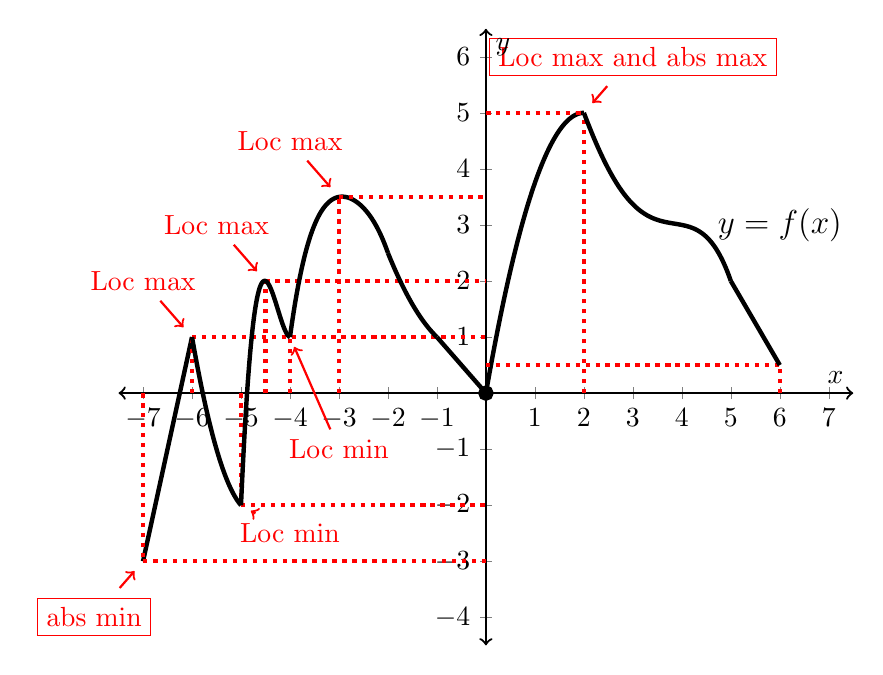
\begin{tikzpicture}
		\begin{axis} [
		width = 0.9\textwidth,
		axis x line=middle,
                   axis y line=middle,
		ymin = -4.5, ymax = 6.5,
		xmin = -7.5, xmax = 7.5,
		xtick={-7, -6, -5, -4, -3, -2, -1, 0, 1, 2, 3, 4, 5, 6, 7},
        		ytick = {-4, -3, -2, -1, 0, 1, 2, 3, 4, 5, 6},
        		xlabel = {$x$},
        		ylabel = {$y$},
        		every axis plot post/.append style={ultra thick},
        		clip = false,
        		axis line style = {<->, thick}
		]
			
			\addplot[mark=*] coordinates {(0,0)};
			
			\addplot [
			black,
			samples = 200,
			domain = -7:-6,
			]
			{((-3*(x+6))/-1)+((1*(x+7))/1)};
			
			\node[red, thick] (source) at (axis cs:-8,-4){\fbox{abs min}};
       			\node (destination) at (axis cs:-7, -3){};
       			\draw[red, thick, ->](source)--(destination);
       			\addplot [red, dotted] coordinates {(-7, 0) (-7, -3)};
       			\addplot[red, dotted, domain = -7:0]{-3};
       			
       			\node[red, thick] (source) at (axis cs:-7,2){Loc max};
       			\node (destination) at (axis cs:-6, 1){};
       			\draw[red, thick, ->](source)--(destination);
       			\addplot [red, dotted] coordinates {(-6, 0) (-6, 1)};
       			\addplot[red, dotted, domain = -6:0]{1};
			
			\addplot [
			black,
			samples = 200,
			domain = -6:-5,
			]
			{((-2*(x+6)*(x+5.5))/0.5)+((1*(x+5)*(x+5.5))/0.5)+((-1*(x+5)*(x+6))/-0.25)};
			
			\node[red, thick] (source) at (axis cs:-4,-2.5){Loc min};
       			\node (destination) at (axis cs:-5, -2){};
       			\draw[red, thick, ->](source)--(destination);
       			\addplot [red, dotted] coordinates {(-5, 0) (-5, -2)};
       			\addplot[red, dotted, domain = -5:0]{-2};
       			
       			\node[red, thick] (source) at (axis cs:-5.5, 3){Loc max};
       			\node (destination) at (axis cs:-4.5, 2){};
       			\draw[red, thick, ->](source)--(destination);
       			\addplot [red, dotted] coordinates {(-4.5, 0) (-4.5, 2)};
       			\addplot[red, dotted, domain = -4.5:0]{2};
			
			\addplot [
			black,
			samples = 200,
			domain = -5:-4,
			]
			{((-2*(x+4.5)*(x+4)*(x+4.25))/-0.375)+((2*(x+5)*(x+4)*(x+4.25))/0.0625)+((1*(x+5)*(x+4.5)*(x+4.25))/0.125)+((1.5*(x+5)*(x+4.5)*(x+4))/-0.046875)};
			
			\node[red, thick] (source) at (axis cs:-3, -1){Loc min};
       			\node (destination) at (axis cs:-4, 1){};
       			\draw[red, thick, ->](source)--(destination);
       			\addplot [red, dotted] coordinates {(-4, 0) (-4, 1)};
			
			\addplot [
			black,
			samples = 200,
			domain = -4:-2,
			]
			{((1*(x+3.5)*(x+3)*(x+2)*(x+2.25))/1.75)+((3*(x+4)*(x+3)*(x+2)*(x+2.25))/-0.46875)+((3.5*(x+4)*(x+3.5)*(x+2)*(x+2.25))/0.375)+((2.5*(x+4)*(x+3.5)*(x+3)*(x+2.25))/0.75)+((3*(x+4)*(x+3.5)*(x+3)*(x+2))/-0.41016)};
			
			\node[red, thick] (source) at (axis cs:-4, 4.5){Loc max};
       			\node (destination) at (axis cs:-3, 3.5){};
       			\draw[red, thick, ->](source)--(destination);
       			\addplot [red, dotted] coordinates {(-3, 0) (-3, 3.5)};
       			\addplot[red, dotted, domain = -3:0]{3.5};
			
			\addplot [
			black,
			samples = 200,
			domain = -2:-1,
			]
			{((2.5*(x+1)*(x+1.75))/0.25)+((1*(x+2)*(x+1.75))/0.75)+((2*(x+2)*(x+1))/-0.1875)};
			
			\addplot [
			black,
			samples = 200,
			domain = -1:-0,
			]
			{((1*(x+0))/-1)+((0*(x+1))/1)};
			
			\addplot [
			black,
			samples = 200,
			domain = 0:2,
			]
			{((5*(x+0)*(x-1))/2)+((0*(x-2)*(x-1))/2)+((3.75*(x-2)*(x+0))/-1)};
			
			\node[red, thick] (source) at (axis cs:3, 6){\fbox{Loc max and abs max}};
       			\node (destination) at (axis cs:2, 5){};
       			\draw[red, thick, ->](source)--(destination);
       			\addplot [red, dotted] coordinates {(2, 0) (2, 5)};
       			\addplot[red, dotted, domain = 0:2]{5};
			
			\addplot [
			black,
			samples = 200,
			domain = 2:5,
			]
			{((5*(x-2.5)*(x-4)*(x-4.75)*(x-5))/8.25)+((4*(x-2)*(x-4)*(x-4.75)*(x-5))/-4.2188)+((3*(x-2)*(x-2.5)*(x-4.75)*(x-5))/2.25)+((2.5*(x-2)*(x-2.5)*(x-4)*(x-5))/-1.1602)+((2*(x-2)*(x-2.5)*(x-4)*(x-4.75))/1.875)};
			\node[black, thick] at (axis cs:6,3){\large$y=f(x)$};
			
       			\addplot [red, dotted] coordinates {(6, 0) (6, 0.5)};
       			\addplot[red, dotted, domain = 0:6]{0.5};
			
			\addplot [
			black,
			samples = 200,
			domain = 5:6,
			]
			{((0.5*(x-5))/1)+((2*(x-6))/-1)};
	\end{axis}
	\end{tikzpicture}
\end{center}
	\pagebreak
\begin{flushleft}
	\textbf{Example 2} \\
	\newline
	For each of the following, determine whether \ul{such a function exists}. If so, provide an example.
	\begin{enumerate}
	\item{ A \ul{continuous function} defined for \ul{all real numbers} \ul{with no absolute extrema}. That is, a continuous function with no absolute maximum and no absolute minimum. \\
	\newline
	\begin{tblr}{
	width=\textwidth, 
	rows = {halign = c, valign = m}, colspec={X Q[c, m] X}}
	{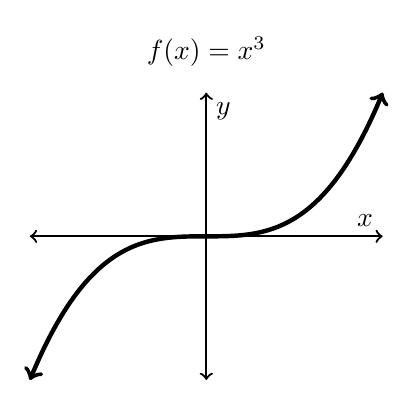
\begin{tikzpicture}
		\begin{axis} [
		width = 0.5\linewidth,
		ticks=none,
		axis x line=middle,
                   axis y line=middle,
		ymin = -8, ymax = 8,
		xmin = -2, xmax = 2,
        		xlabel = {$x$},
        		ylabel = {$y$},
        		every axis plot post/.append style={ultra thick, <->},
        		clip = false,
        		axis line style = {<->, thick},
        		title = {$f(x) = x^3$},
		]
			\addplot [
			black,
			samples = 200,
			domain = -2:2
			]
			{x^3};
	\end{axis}
	\end{tikzpicture}} & or &
	{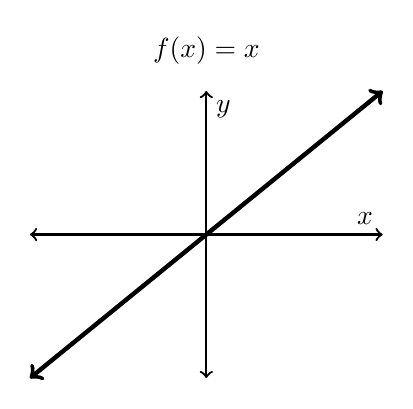
\begin{tikzpicture}
		\begin{axis} [
		width = 0.5\linewidth,
		ticks=none,
		axis x line=middle,
                   axis y line=middle,
		ymin = -2, ymax = 2,
		xmin = -2, xmax = 2,
        		xlabel = {$x$},
        		ylabel = {$y$},
        		every axis plot post/.append style={ultra thick, <->},
        		clip = false,
        		axis line style = {<->, thick},
        		title = {$f(x) = x$},
		]
			\addplot [
			black,
			samples = 200,
			domain = -2:2,
			]
			{x};
	\end{axis}
	\end{tikzpicture}} \\
	\end{tblr} \begin{center} No abs max and no abs min \end{center}}
	\item{A \ul{function} defined on the closed \ul{interval $[0, 1]$} with no \ul{absolute maximum} and \ul{no absolute minimum}. \\
	\begin{center}
	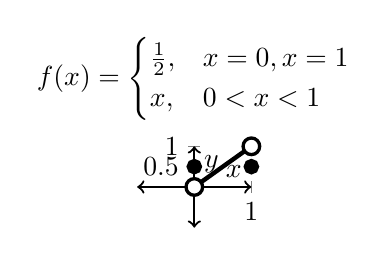
\begin{tikzpicture}
		\begin{axis} [
		width = 0.25\linewidth,
		axis x line=middle,
                   axis y line=middle,
		ymin = -1, ymax = 1,
		xmin = -1, xmax = 1,
		xtick = {0, 1},
		ytick = {1/2, 1},
        		xlabel = {$x$},
        		ylabel = {$y$},
        		every axis plot post/.append style={ultra thick},
        		clip = false,
        		axis line style = {<->, thick},
        		title = {{$\displaystyle{f(x)=\begin{cases} \frac{1}{2}, & x=0, x=1 \\ x, & 0<x<1\end{cases}}$}},
		]
			\addplot [
			black,
			samples = 200,
			domain = 0:1,
			]
			{x};
		\fill[white,draw=black, very thick](axis cs:0,0)circle[radius=3pt];
		\fill[white,draw=black, very thick](axis cs:1,1)circle[radius=3pt];
		
		\addplot[mark=*] coordinates {(0,1/2)};
		\addplot[mark=*] coordinates {(1,1/2)};
	\end{axis}
	\end{tikzpicture} \\
	No abs max and no abs min \end{center}}
	\item{ A \ul{\textbf{continuous} function} defined on the \ul{closed interval $[0, 1]$} with no \ul{absolute maximum} and \ul{no absolute minimum}. \\
	\newline
	Impossible to find continuous function defined in close interval without abs max and abs min \\
	\begin{center}
	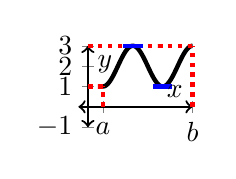
\begin{tikzpicture}
		\begin{axis} [
		width = 0.25\linewidth,
		axis x line=middle,
                   axis y line=middle,
		ymin = -1, ymax = 3,
		xmin = -1, xmax = 7*pi / 2,
		xtick = {pi/2,  7*pi/2},
        		xlabel = {$x$},
        		ylabel = {$y$},
        		every axis plot post/.append style={ultra thick},
        		clip = false,
        		axis line style = {<->, thick},
        		xticklabels={$a$, $b$}
		]
			\addplot [
			black,
			samples = 200,
			domain = pi/2:7*pi / 2,
			]
			{cos(deg(x+pi/2))+2};
			
			\addplot [red, dotted] coordinates {(pi/2, 0) (pi/2, 1)};
       			\addplot[red, dotted, domain = 0:pi/2]{1};
       			
       			\addplot [red, dotted] coordinates {(7 *pi/2, 0) (7 *pi/2, 3)};
       			\addplot[red, dotted, domain = 0:7 * pi/2]{3};
       			
       			\addplot[blue, domain = 3 * pi/2 - 1:3 * pi/2 + 1]{3};
       			\addplot[blue, domain = 5 * pi/2 - 1:5 * pi/2 + 1]{1};
	\end{axis}
	\end{tikzpicture}
	\end{center}
	}
	\end{enumerate}
	\fbox{
	\parbox{\textwidth}{
	\newline
		\textbf{The Extreme Value Theorem} \\
		\newline
		If $f$ is \ul{continuous} on a closed interval $[a, b]$, then $f$ attains an \ul{absolute maximum value
$f(c)$} and an \ul{absolute minimum value $f(d)$} at\ul{ some numbers $c$ and $d$ in $[a, b]$}.\\}} \\
\newline
\textbf{Note: }  The EVT does \textbf{NOT} say where these values are located.
\end{flushleft}
\end{document}